%図は改良の余地あり

\chapter{背景}

本章では、多層パーセプトロン及びその応用例であるGenerative~Adversarial~Networks~(GAN)~の説明を行った後にGANを画像のスタイル変換に応用したPix2pixを紹介する。

%ニューラルネットはこの前まででなんとなく説明しておく!
\section{Multilayer~perceptron}

Multilayer~perceptron~(多層パーセプトロン)~はニューラルネットワークの一つである。

%ここから数式(メモは済)

\subsection{層と活性化関数}

%入力層と出力層と隠れ層を持つ
%行列と活性化関数の演算
%活性化関数により非線形分離


\subsection{誤差関数と誤差逆伝播法}

%任意の活性化関数は微分可能
%誤差関数
%誤差逆伝播

\section{GAN}

\begin{figure}[H]
\begin{center}
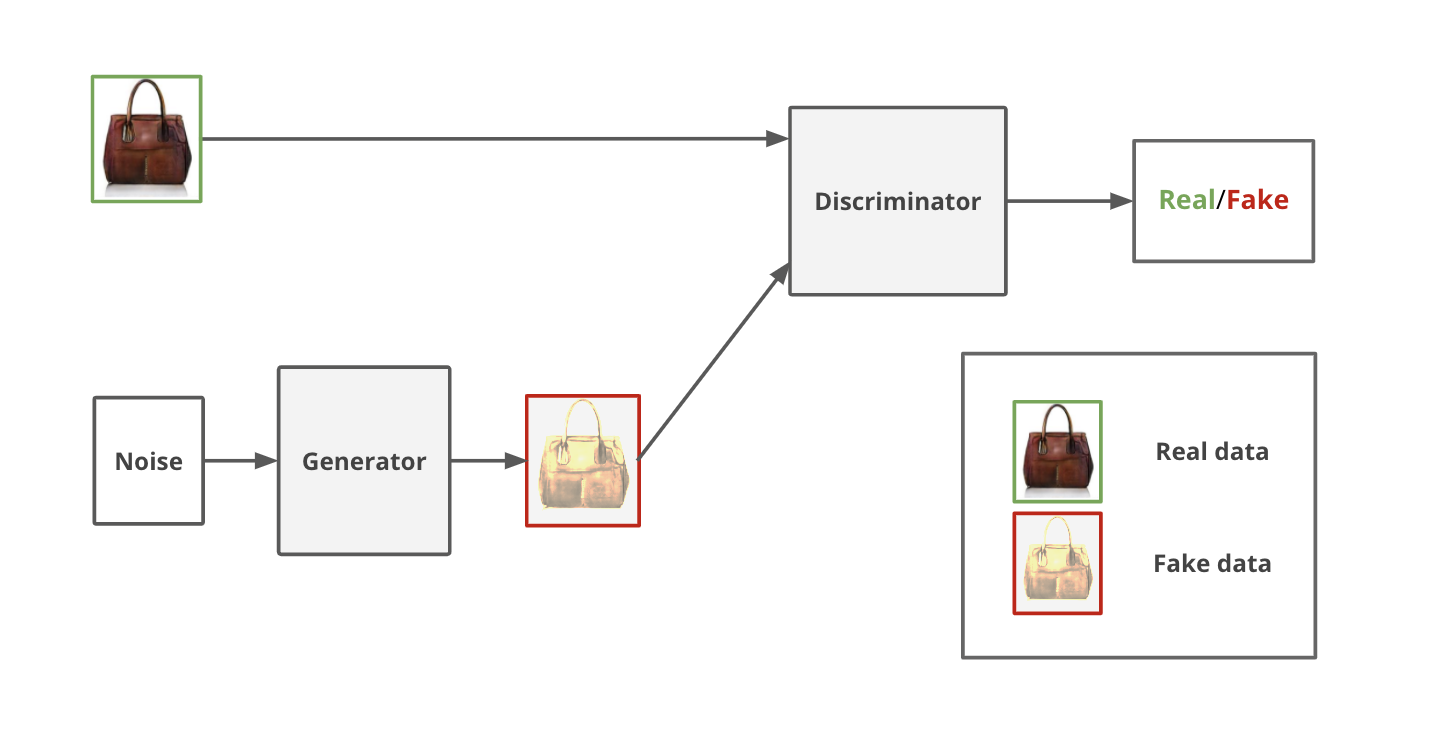
\includegraphics[width=\hsize]{figure/GAN_net.png}
\caption{GANのネットワークの図}
\label{fig:GAN_net}
\end{center}
\end{figure}


GAN~\cite{GAN}は多層パーセプトロンの応用例であり、生成モデルと識別モデルが競合して学習を行う。生成モデルは自身の出力が学習データであると識別モデルに推定させること、識別モデルは学習データと生成モデルの出力のどちらであるかを正しく推定することを目指して学習する。

また、生成モデルの目的関数は式\ref{eq:GAN_G}であり、識別モデルの目的関数は\ref{eq:GAN_D}である。

\begin{align}
    \label{eq:GAN_G}
    \argmin _{\theta_G}& \mathbb{E}_{\boldsymbol{z}}[\log (1-D(G(\boldsymbol{z};\theta_G);\theta_D))]\\
    \label{eq:GAN_D}
    \argmax _{\theta_D}& \mathbb{E}_{\boldsymbol{x}}[\log D(\boldsymbol{x};\theta_D)]+\mathbb{E}_{\boldsymbol{z}}[\log (1-D(G(\boldsymbol{z};\theta_G);\theta_D))]
\end{align}

ここで、$\boldsymbol{x}$は学習データ,$\boldsymbol{z}$は生成モデルへの入力のノイズ,$G(\boldsymbol{z};\theta_G)$はノイズ$\boldsymbol{z}$を入力とする生成モデル,$D(\cdot;\theta_D)$は識別モデル,$\theta_G$は生成モデル$G$のパラメータ,$\theta_D$は識別モデル$D$のパラメータである。



\section{Pix2pix}

\begin{figure}[H]
\begin{center}
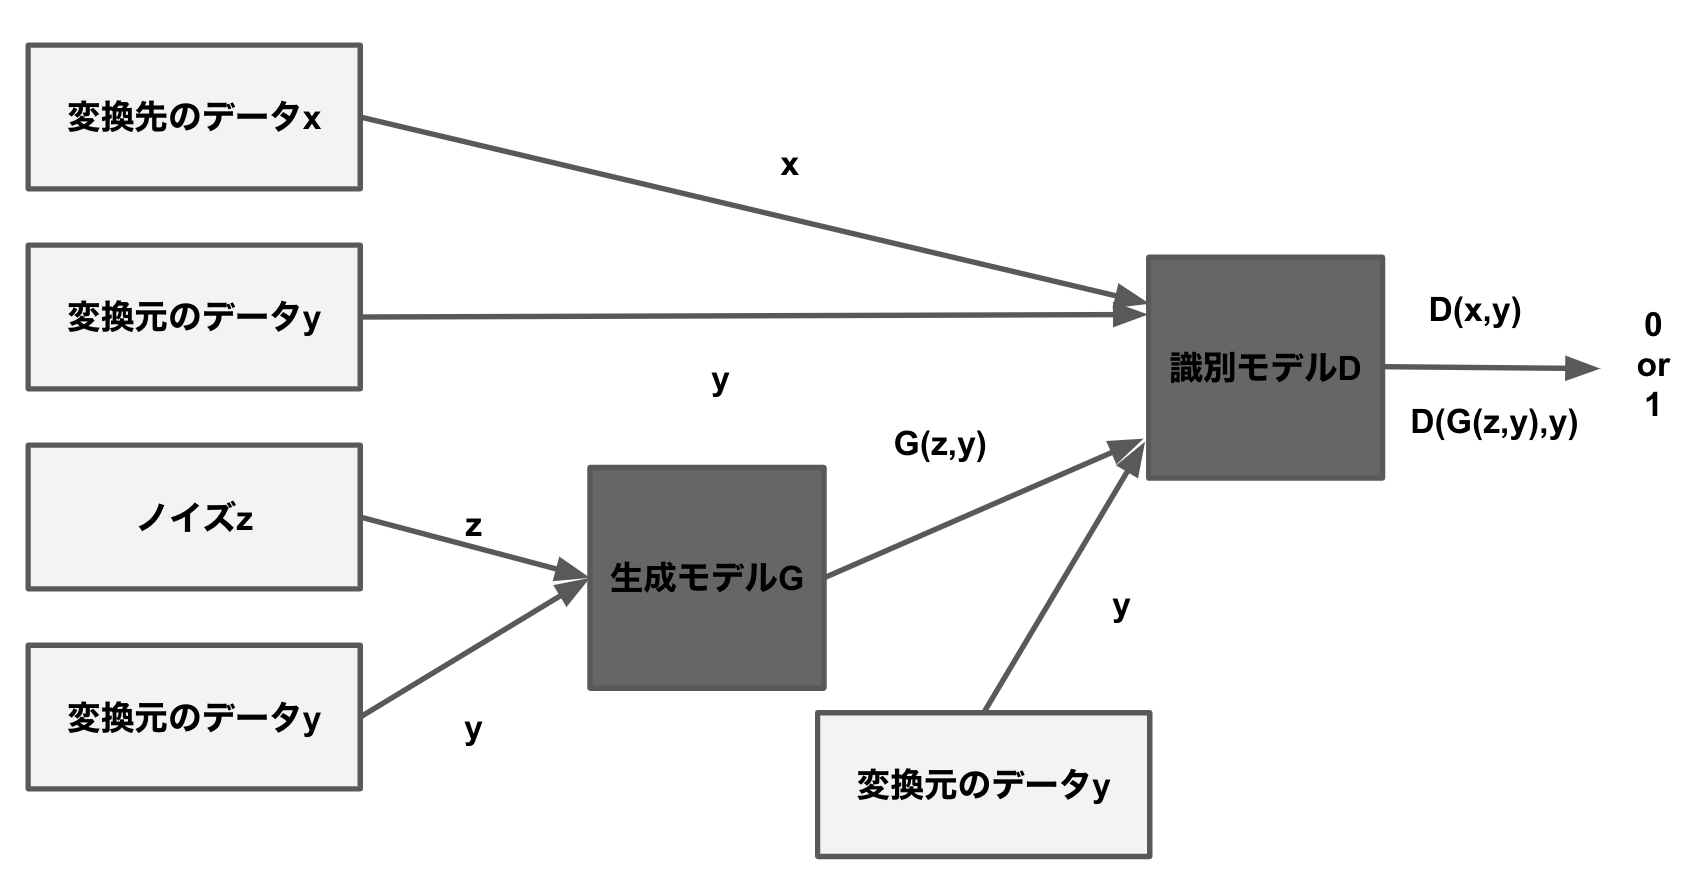
\includegraphics[width=\hsize]{figure/pix2pix_net.png}
\caption{pix2pixのネットワークの図}
\label{fig:pix2pix_net}
\end{center}
\end{figure}

Pix2pix~\cite{pix2pix}はある条件下で画像間の変換を行うGANである。図\ref{fig:pix2pix_img}にあるようにピクセルの対応関係を変えずにスタイル変換を行うことができる。

\begin{figure}[t]
\begin{center}
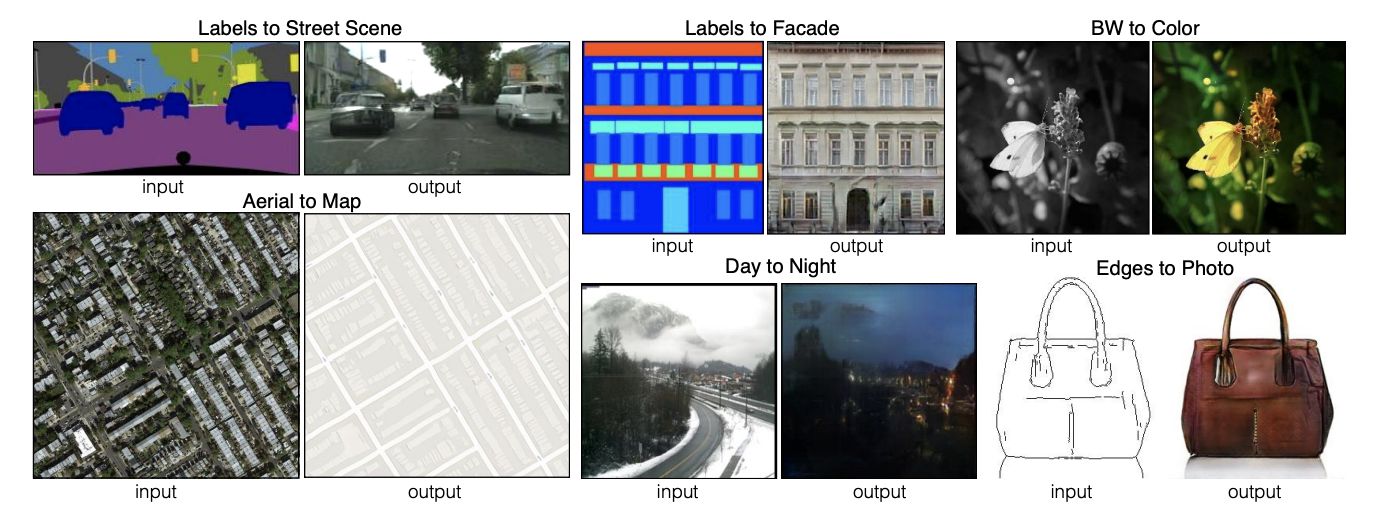
\includegraphics[width=\hsize]{figure/pix2pix_img.png}
\caption{pix2pixのスタイル変換の例}
\label{fig:pix2pix_img}
\end{center}
\end{figure}

また、生成モデルの目的関数は式\ref{eq:pix2pix_G}であり、識別モデルの目的関数は\ref{eq:pix2pix_D}である。このような条件付きのGANをConditional~GAN~\cite{CGAN}と呼ぶ。

\begin{align}
    \label{eq:pix2pix_G}
    \argmin _{\theta_G}& \mathbb{E}_{\boldsymbol{x}, \boldsymbol{z}}[\log (1-D(\boldsymbol{x}, G(\boldsymbol{x}, \boldsymbol{z}; \theta_G); \theta_D))]+\mathbb{E}_{\boldsymbol{x}, \boldsymbol{y}, \boldsymbol{z}}[\|\boldsymbol{y}-G(\boldsymbol{x}, \boldsymbol{z}; \theta_G)\|_{1}]\\
    \label{eq:pix2pix_D}
    \argmax _{\theta_D}& \mathbb{E}_{\boldsymbol{x}, \boldsymbol{y}}[\log D(\boldsymbol{x}, \boldsymbol{y}; \theta_D)]+\mathbb{E}_{\boldsymbol{x}, \boldsymbol{z}}[\log (1-D(\boldsymbol{x}, G(\boldsymbol{x}, \boldsymbol{z}; \theta_G); \theta_D))]
\end{align}


ここで、$\boldsymbol{x}$は変換先の学習データ,$\boldsymbol{y}$は変換元の学習データ,$\boldsymbol{z}$は生成モデルへの入力のノイズ,$G(\boldsymbol{x},\boldsymbol{z};\theta_G)$はノイズ$\boldsymbol{z}$を入力とする生成モデル,$D(\boldsymbol{x},\cdot;\theta_D)$は識別モデル,$\theta_G$は生成モデル$G$のパラメータ,$\theta_D$は識別モデル$D$のパラメータである。

\subsection{生成モデルの構造}

\begin{figure}[H]
\begin{center}
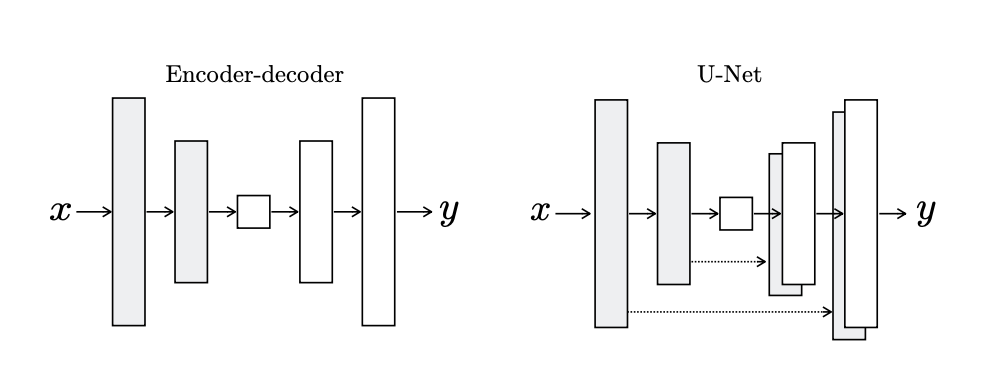
\includegraphics[width=\hsize]{figure/u-net.png}
\caption{U-netのネットワーク}
\label{fig:u-net}
\end{center}
\end{figure}

%説明が雑すぎる

生成モデルはスタイル変換を行うために全体的な構造を維持する必要があり、encoder-decoderのネットワークとして\ref{fig:u-net}のようなU-net\cite{u-net}におけるスキップコネクションブロックが用いられる。

\subsection{識別モデルの構造}

\textcolor{red}{3.2.2の内容をまとめる}


